\begin{center}
    \section*{BAB 4 HASIL KERJA}
\end{center}

\setcounter{section}{4}
\setcounter{subsection}{0}

%\subsection{Hasil Kerja}
    Hasil kerja yang kami hasilkan adalah berupa produk yang dapat diimplementasikan di kehidupan nyata. Produk ini dapat diimplementasikan ke telur yang dapat menetas. Kami menggunakan box sterefoam sebagai closure. Di dalam sterefoam, kami memasukkan semua alat yang dibutuhkan seperti yang telah dijelaskan pada pembahasan. Cara kerja dari alat ini adalah meletakkan telur di dalam sterefoam. Sensor suhu sangat berperan dan berpengaruh ke alat yang kami kerjakan. Ketika sensor mendeteksi perubahan suhu, salah satu dari dua aktuator akan bekerja. Lampu dan kipas dapat dikendalikan oleh program dari esp32 dan sensor suhu yang sangat berperan sekali pada produk yang kami gunakan ini. Berikut adalah foto hasil produk yang sudah jadi:

    \begin{figure}[h]
    \centering
    \begin{minipage}{.48\textwidth}
        \centering
        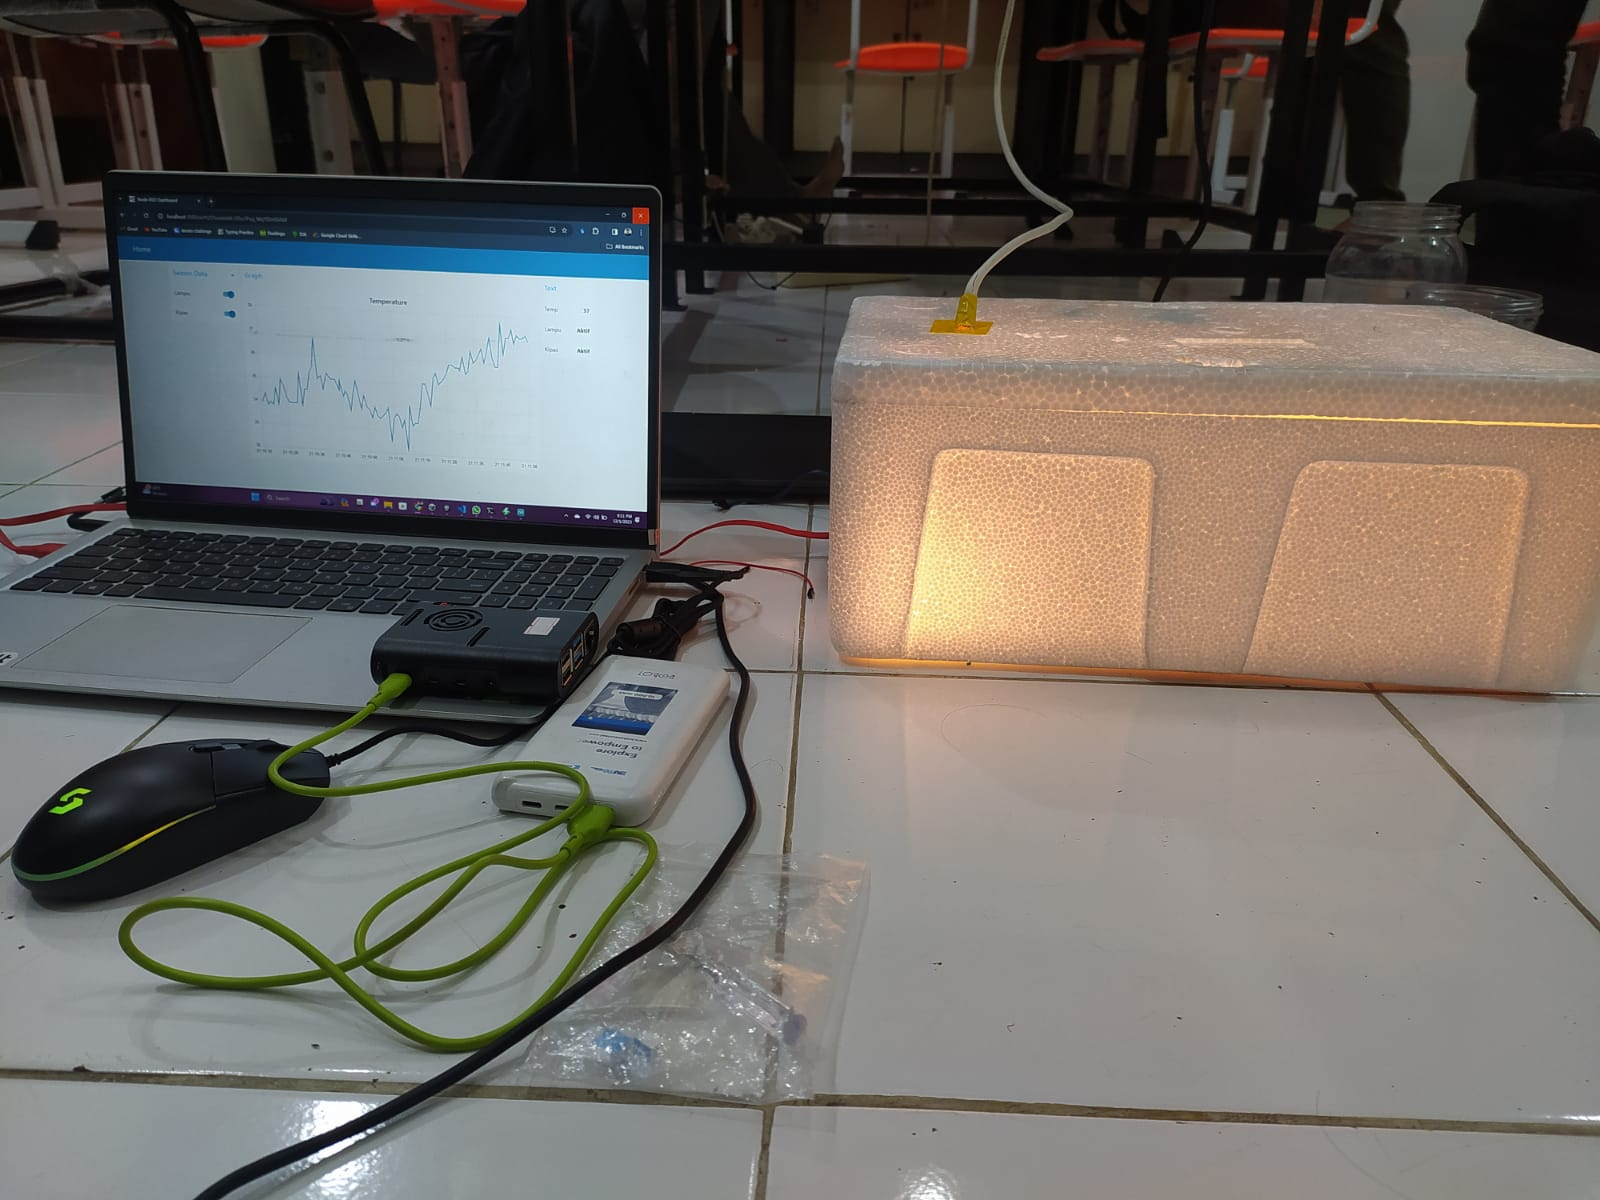
\includegraphics[width=\linewidth]{image/foto_alat1.jpg}
        \caption{Alat tampak depan}
        \label{fig:gambar-kiri}
    \end{minipage}
    \hfill
    \begin{minipage}{.48\textwidth}
        \centering
        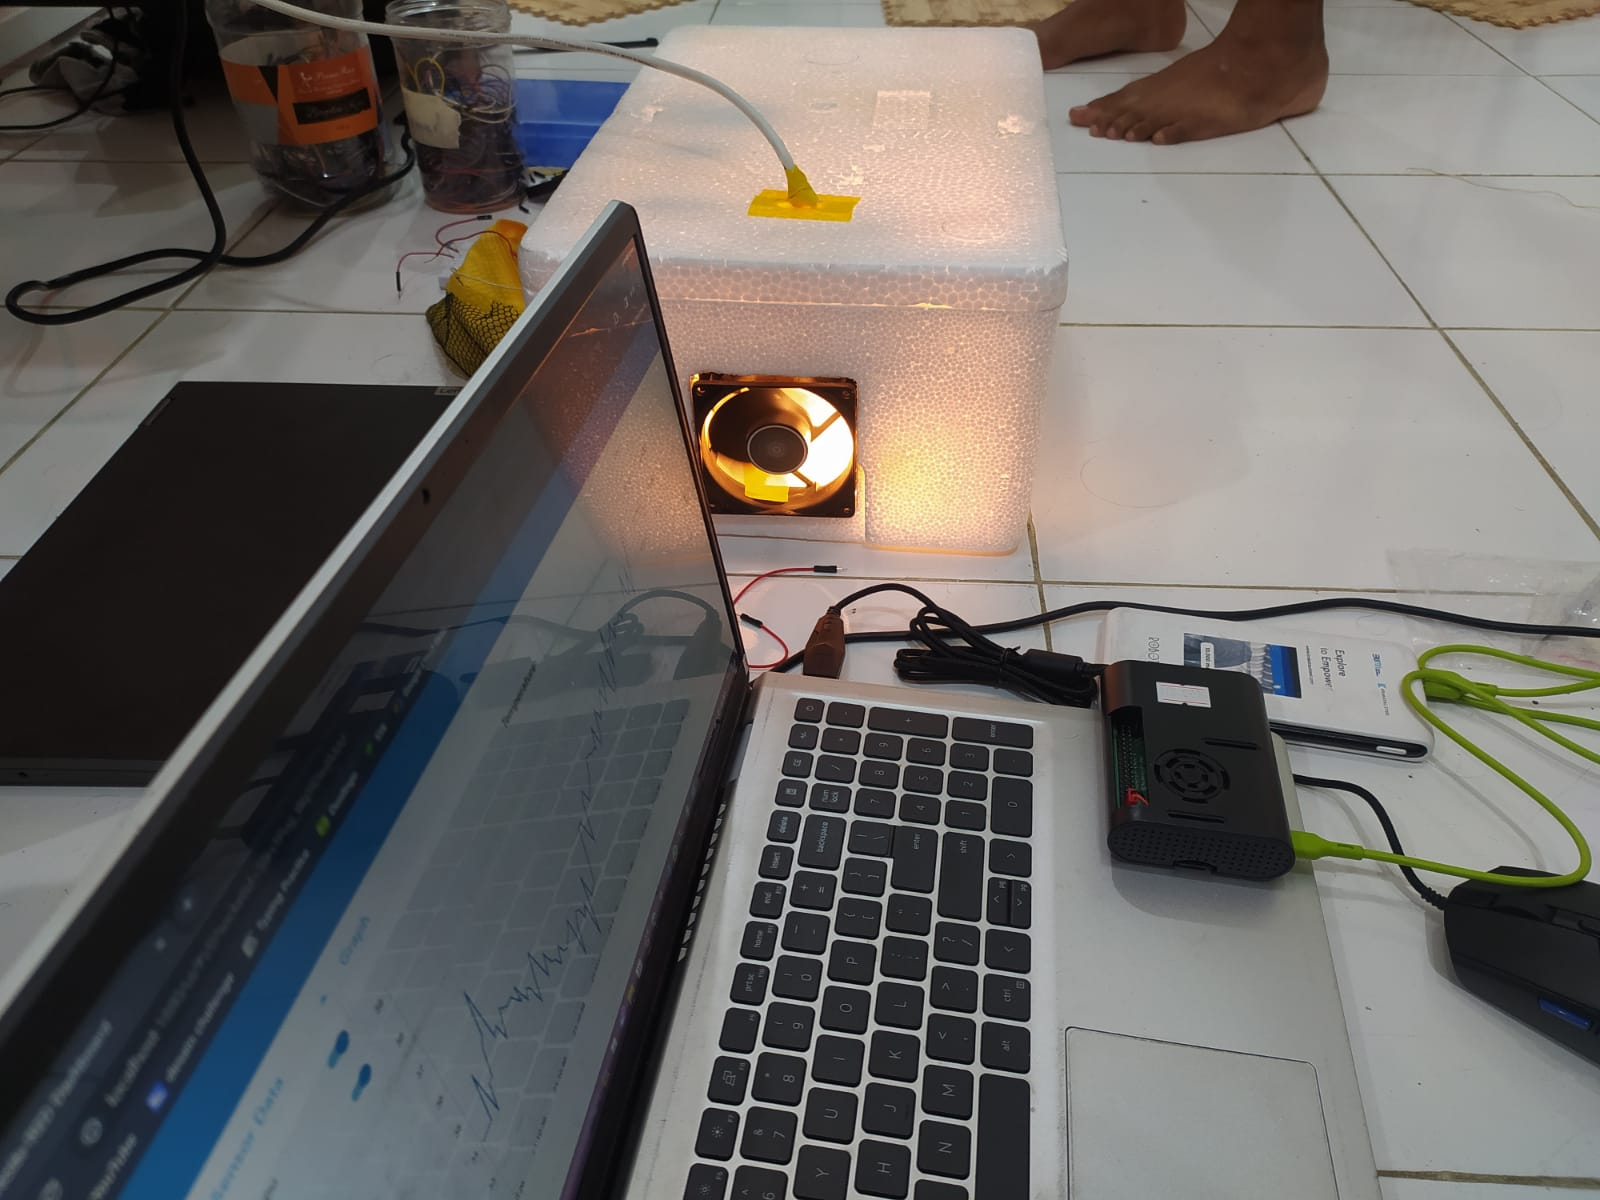
\includegraphics[width=\linewidth]{image/foto_alat2.jpg}
        \caption{Alat tampak samping}
        \label{fig:gambar-kanan}
    \end{minipage}
\end{figure}

%\subsection{ESP-32 Program}
Berikut adalah listing program yang digunakan menggunakan platform Arduino IDE:
\lstinputlisting{Program/mqtt_tes_2.ino}